% !TEX root = algo-quicksheet.tex
\chapter{Math}

\section{Functions}
\rih{Equals.} Requirements for equals
\begin{enumerate}
\item Reflexive
\item Symmetric
\item Transitive
\item Non-null
\end{enumerate}
\rih{Compare.} Requirements for compares (total order):
\begin{enumerate}
\item Antisymmetry
\item Transitivity
\item Totality
\end{enumerate}
\section{Divisor}
\runinhead{gcd.} Greatest common divisor.
$$
gcd(a,b) = gcd(b, r)
$$
\begin{center}
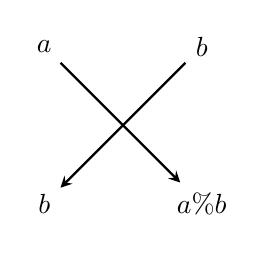
\begin{tikzpicture}[->, thick, >=stealth]

% Nodes
\node (a) at (0,2) {\(a\)};
\node (b) at (2,2) {\(b\)};
\node (mod) at (2,0) {\(a \% b\)};
\node (b2) at (0,0) {\(b\)};

% Arrows
\draw (a) -- (mod);
\draw (b) -- (b2);

\end{tikzpicture}
\end{center}

\begin{python}
# recursive abbr
def gcd(a, b):
    if b == 0:
        return a
        
    return gcd(b, a % b)

# iterative     
def gcd(a, b):
    while b != 0:
        a, b = b, a % b

    return a
\end{python}

\rih{Proof}. Euclidean Algorithm. The Euclidean algorithm is based on the principle that the GCD of two numbers $a$ and $b$ is the same as the GCD of $b$ and $a\%b$ until $b$ becomes zero. Prove the following recursive form:
$$
gcd(a,b) = gcd(b, r)
$$
\begin{enumerate}
\item \rih{Divisibility}: Let $g$ be the GCD of $a$ and $b$. By definition, $g$ divides both $a$ and $b$. From the equation $a=b\cdot q+r$, it follows that $g$ must also divide the remainder $r$, because any divisor of both $a$ and $b$ divides linear combination of them: $r = a - b \cdot q$. 
\item \rih{Reduction}: If we replace $a$ with $b$ and $b$ with $r$, the GCD remains unchanged, and the problem size gets smaller (since $r<b$). 
\item \rih{Termination}: The algorithm repeatedly reduces the size of the numbers by replacing the larger number with the remainder. Eventually, one of the numbers will become zero, and the GCD is the other number, since $gcd(a,0)=a$.
\end{enumerate}
\section{Power}
\runinhead{power(x, n).} To calculate $x^n$. 
\runinhead{Core Clues}:
\begin{enumerate}
\item $O(N)$ is trivial, need to do better than it
\item Divide the problem by half
\begin{align*}
x^n &= (x^2)^{n/2} \\
x^n &= x^{n/2} * x^{n/2} * x^{n \mod 2}
\end{align*}
\end{enumerate}
\begin{python}
def pow(self, x, n):
    is_invert = False if n > 0 else True

    n = abs(n)
    ret = 1.0
    while n > 0:
        if n & 1 == 1:
            ret *= x

        n >>= 1
        x *= x

    if is_invert:
        ret = 1.0 / ret

    return ret
\end{python}
\section{Prime Numbers}
\subsection{Sieve of Eratosthenes}
\subsubsection{Basics}
To find all the prime numbers less than or equal to a given integer n by Eratosthenes' method:
\begin{enumerate}
\item Create a   list of consecutive integers from 2 through n: (2, 3, 4, ..., n).
\item Initially, let $p$ equal 2, the first prime number.
\item Starting from $p$, enumerate its multiples by counting to n in increments of  $p$, and mark them in the list (these will be $2p$, $3p$, $4p$, ... ; the $p$ itself should not be marked).
\item Find the first number greater than $p$ in the list that is not marked. If there was no such number, stop. Otherwise, let $p$ now equal this new number (which is the next prime), and repeat from step 3.
\end{enumerate}

When the algorithm terminates, the numbers remaining not marked in the list are all the primes below $n$.

\subsubsection{Refinements}
The main idea here is that every value for $p$ is prime, because we have already marked all the multiples of the numbers less than $p$. Note that some of the numbers being marked may have already been marked earlier (e.g., 15 will be marked both for 3 and 5).

As a refinement, it is sufficient to mark the numbers in step 3 starting from $p^2$, because all the smaller multiples of $p$ will have already been marked at that point by the previous smaller prime factor other than $p$. From $p^2$, $p$ becomes the smaller prime factor of a composite number. This means that the algorithm is allowed to terminate in step 4 when $p^2$ is greater than n.

For example, consider $p=5$. The first multiple of 5 that we need to mark is $5^2 = 25$, because: 
\begin{enumerate}
\item $5 \times 2 = 10$ has already been marked when processing $p = 2$.
\item $5 \times 3 = 15$ has already been marked when processing $p = 3$ 
\item $5 \times 4 = 20$ has already been marked when processing $p = 2$. 
\end{enumerate}
Therefore, we only need to start marking multiples from $p^2$, since all smaller multiples of $p$ have already been handled.

\begin{python}
def count_primes_sieve(N):
    if N < 2:
        return 0
    # intialize all numbers prime candidates
    primes = [True for _ in range(N+1)]
    # 0 and 1 are not prime numbers
    primes[0] = primes[1] = False

    p = 2
    while (p * p <= N):
        if primes[p]:
            for i in range(p * p, N+1, p):
                primes[i] = False
        p += 1

    return sum(prime)
\end{python}

\rih{Time complexity}. Iterating \pyinline{p} is $O(N)$ and for all the prime number, each inner loop take $\frac{N}{p}$. Then it becomes 

$$
\sum_{p \leq N} \frac{N}{p} = N \sum_{p \leq N} \frac{1}{p}
$$

It looks like $O(N \log N)$ but $p$ are prime numbers, it becomes $O(N \log \log N)$. The \rih{Prime Number Theorem} tells us that the number of primes less than or equal to $N$ is approximate
$$
\frac{N}{\log N}
$$


Another refinement is to initialize list odd numbers only, (3, 5, ..., n), and count in increments of $2p$ in step 3, thus marking only odd multiples of $p$. This actually appears in the original algorithm. This can be generalized with wheel factorization, forming the initial list only from numbers coprime with the first few primes and not just from odds (i.e., numbers coprime with 2), and counting in the correspondingly adjusted increments so that only such multiples of $p$ are generated that are coprime with those small primes, in the first place.



To summarized, the refinements include:
\begin{enumerate}
\item Starting from $p^2$; thus $p$ is the smaller prime factor. 
\item Preprocessing even numbers and then only process odd numbers; thus the increment becomes $2p$.
\end{enumerate}

\begin{python}
def count_primes(N):
    if N < 3:
        return 0
    primes = [
        False if i%2 == 0 else True 
        for i in range(n)
    ]
    primes[0], primes[1] = False, False
    for i in range(3, int(math.sqrt(N))+1, 2):
        if primes[i]:
            for j in range(i*i, n, 2*i):
                primes[j] = False

    return prime.count(True)
\end{python}

\subsection{Factorization}
Backtracking: Section-\ref{factorization}.

\section{Median}
\subsection{Basic DualHeap}
\runinhead{Sliding Window Median.} Find the list of median in the sliding window. $\Ra$ Dual heap with lazy deletion.

DualHeap to keep track the median when a method to find median is called multiple times.

Here we use the negation of the value as a trick to convert min-heap to max-heap.
\begin{python}
import heapq

class DualHeap:
  def __init__(self):
    self.min_h = []
    self.max_h = []  # need to negate the value 

  def insert(self, num):
    if not self.min_h or num > self.min_h[0]:
      heapq.heappush(self.min_h, num)
    else:
      heapq.heappush(self.max_h, -num)
    self.balance()

  def balance(self):
    l1 = len(self.min_h)
    l2 = len(self.max_h)
    if l1-l2 > 1:
      heapq.heappush(self.max_h, 
                     -heapq.heappop(self.min_h))
      self.balance()
    elif l2-l1 > 1:
      heapq.heappush(self.min_h, 
                     -heapq.heappop(self.max_h))
      self.balance()
    return

  def get_median(self):
    """Straightforward"""
\end{python}

\subsection{DualHeap with Lazy Deletion}\label{dh_lazy_del}
Clues:
\begin{enumerate}
\item Wrap the value and wrap the heap
\item When delete a value, mark it with tombstone. 
\item When negate the value, only change the value, not the reference. 
\item When heap pop, clean the op first. 
\end{enumerate}
\begin{python}
import heapq
from collections import defaultdict
from dataclasses import dataclass

@dataclass
class Value:
    val: int
    deleted: bool


class Heap:
    def __init__(self):
        self.h = []
        self.len = 0

    def push(self, item):
        heapq.heappush(self.h, item)
        self.len += 1

    def pop(self):
        self._clean_top()
        self.len -= 1
        return heapq.heappop(self.h)

    def remove(self, item):
        """lazy delete"""
        item.deleted = True
        self.len -= 1

    def __len__(self):
        return self.len

    def _clean_top(self):
        while self.h and self.h[0].deleted:
            heapq.heappop(self.h)

    def peek(self):
        self._clean_top()
        return self.h[0]


class DualHeap:
    def __init__(self):
        self.min_h = Heap()  # represent right side
        self.max_h = Heap()  # represent left side
    # others similar as the previous section's above DualHeap
\end{python}

\section{Modular}
\subsection{Power of 4}
To check whether a number of the power of 4, we can check whether it mod 3 equals 1.
\begin{align*}
4^a &\equiv 1^a\mod 3 \\
&\equiv 1 \mod 3
\end{align*}

Alternatively, we can use bit manipulation based on the power of 4 in the binary form of \pyinline{repeat n 1 << 2}, and checks whether there is even number of 0's in binary form. 

\section{Ord}
\runinhead{Number in lexical order.} Given an integer n, return 1 ~ n in lexicographical order. For example, given 13, return: [1,10,11,12,13,2,3,4,5,6,7,8,9].

Enumerate to find the pattern:
\begin{python}
1	10	11	...	19
2	21	22	...	29
3	31	32	...	39
4 ...
.
.
\end{python}

Using DFS.
\begin{python}
def dfs(cur, ret, N):
    ret.append(cur)
    for d in range(10):
        nxt = cur * 10 + d
        if nxt <= N:
            dfs(nxt, ret, N)
        else:
            break

N = 105
ret = []
for i in range(1, 10):
    if i <= N:
        dfs(i, ret, N)
    else:
        break
\end{python}

Optionally, using iterative appraoch. 
\begin{python}
def gen():
    i = 1
    for _ in range(n):
        yield i
        if i * 10 <= n:
            i *= 10  # * 10
        elif i % 10 != 9 and i + 1 <= n:
            i += 1  # for current digit
        else:
            while i % 10 == 9 or i + 1 > n:
                i //= 10
            i += 1
\end{python}
